\chapter{Support Vector Machines And Kernel Method}
\label{ch-svm}
This chapter is based on Refs.\cite{wiki-kernel-way}.
\cite{wiki-svm} and \cite{wiki-kernel-per}.

The Support Vector Machines (SVM) method
was first invented with a linear kernel, but
was later generalized to arbitrary kernels.
We will use the terms SVM method and Kernel Method
indistinguishably. 

The SVM method is a
fairly general method
for
calculating, via supervised learning, a
{\it binary} classifier.
The SVM method
finds a continuous surface
that separates a space into two 
disjoint parts.


Let $\Sigma=[0,1,2, \ldots, nsam-1]$ be a list of
individuals (samples) in a population.
In this chapter, we will use the notation 
$A^\s=A[\s]$ 
and $\vec{A}=[A^\s:\s\in \Sigma]$
for a  list (vector, 1-D  array) 
indexed by $\Sigma$.
We will refer to $DS=(\vec{x}, \vec{y})$ 
where $x^\s\in S_\rvx$,
 $y^\s\in \{-1, 1\}$,
as a dataset. Let
$x^\s=(x^\s_0, x^\s_1, 
\ldots, x^\s_{nf-1})
\in S_{\rvx_0}\times S_{\rvx_1}
\times\ldots\times
 S_{\rvx_{nf-1}}=S_\rvx$.
When $x^\s_j\in \RR$ for all 
$j$,
we will take $x^\s\in \RR^{nf}$ 
to be a column vector.
$x^\s$ is the feature vector for individual
$\s$, and its components $x^\s_i$
for $i=0,1,\ldots, nf-1$ are the features.
$y^\s\in \{-1, 1\}$ is the binary 
class to which $x^\s$ belongs.

Let $\haty(x^{\s_0})\in\{-1, 1\}$ be an estimate of
$y^{\s_0}\in\{-1, 1\}$.
The {\bf SVM classifier} is defined as

\beq
\haty(x^{\s_0})=\sign(Y(x^{\s_0}))
\label{eq-svm-haty}
\eeq
where\footnote{Define $\sign(0)=1$.}

\beq
Y(x^{\s_0})=\sum_\s
\alp^\s y^\s 
K(x^\s, x^{\s_0})
\;.
\label{eq-yy-x-sig}
\eeq
The {\bf binary weight coefficients} $\alp^\s\in \bool$
for all $\s\in\Sigma$ are found 
by training, via an algorithm
to be described below.

The function $K:S_\rvx\times S_\rvx
\rarrow \RR$
is called the {\bf Kernel 
or Similarity function}.
We assume that
$K(x^\s, x^{\s_0})$ grows bigger
when its two arguments
$x^\s$ and $x^{\s_0}$ 
become more ``similar".
We
also assume that
$K(x^\s, x^{\s_0})$ is symmetric in its two arguments.

\section{Learning Algorithm for SVM Classifier}



\begin{figure}[h!]
$$
\xymatrix{
&\vec{\ul{\alp}}\ar@/^1.5pc/[dd]
\ar[r]
&\vec{\ul{\alp}'}\ar@/^1.5pc/[dd]
\\
&\rvx^{\s_0}\ar@/^1pc/[d]
&\rvx^{\s_0+1}\ar@/^1pc/[d]
\\
(\vec{\rvx}, \vec{\rvy})\ar[r]
\ar@/_1pc/[rr]
&\ul{\haty}\ar[d]
&\ul{\haty}'\ar[d]
\\
&\ul{\cale}\ar[ruuu]
&\ul{\cale'}
\\
&\rvy^{\s_0}\ar[u]
&\rvy^{\s_0+1}\ar[u]
}
$$
\caption{Time slice $\s_0$ of dynamical bnet for
learning binary weights $\vec{\alp}$ 
of SVM classifier.
}
\label{fig-svm-bnet}
\end{figure}

Given a kernel function $K$ and a dataset 
$(\vec{x}, \vec{y})$,
the SVM classifier is fully specified
except for its binary weights $\vec{\alp}$.
Those weights can be learned via 
the algorithm
represented as a causal diagram  in Fig.\ref{fig-svm-bnet}.
That figure  shows one time slice
of a dynamical bnet.
The TPMs, printed in blue,
of bnet Fig.\ref{fig-svm-bnet},
are as follows:



\beq\color{blue}
P(\haty|\vec{\alp}, (\vec{x},\vec{y}), x^{\s_0})
=
\indi(\;\;\;
\haty= \text{ given by Eq.(\ref{eq-svm-haty}).}
\;\;\;)
\eeq  

\beq\color{blue}
P(\cale| \haty, y^{\s_0})
=
\indi(\;\;\;\cale =
\indi(\haty\neq y^{\s_0})
\;\;\;)
\eeq  

The first (but not the second, third , etc.)
$\vec{\alp}$ 
node of Fig.\ref{fig-svm-bnet}
is a root node.
The TPM for that root node
should set 
all components of $\vec{\alp}$
to zero:

\beq\color{blue}
P(\vec{\alp})=\prod_\s \indi(\;\;\;
\alp^\s=0
\;\;\;)
\;.
\eeq
After that initialization,
\beq\color{blue}
P(\vec{\alp'}|\vec{\alp}, \cale)=
\indi(\;\;\;(\alp')^{\s_0}=\alp^{\s_0} +\cale\;\;\;)\;\;
\prod_{\s\neq \s_0}
\indi(\;\;\;(\alp')^\s=\alp^\s
\;\;\;)
\eeq

\noindent {\bf Why this learning algorithm works.}
\begin{figure}[h!]
\centering
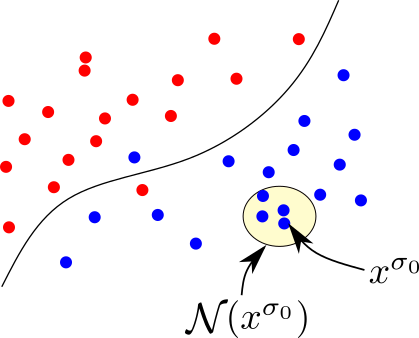
\includegraphics[width=2in]
{svm/svm-why.png}
\caption{Define the neighborhood
of $x^{\s_0}$ by  $\caln(x^{\s_0})
=
\{x^\s: |K(x^\s,  x^{\s_0})|<\eps \}$
for some $\eps>0$.}
\label{fig-svm-why}
\end{figure}

$K(x^\s, x^{\s_0})$
sets to zero any contribution to
$Y(x^{\s_0})$
from points $x^\s$
outside the 
neighborhood $\caln(x^{\s_0})$
of $x^{\s_0}$.
 (See Fig.\ref{fig-svm-why}).
If $\haty(x^{\s_0})=y^{\s_0}$,
keep
$\alp^{\s_0}=0$ because
the 
neighbors of $x^{\s_0}$
are giving the correct 
$\haty(x^{\s_0})$
when they are polled 
and the majority wins.
If,
on the other hand,
 $\haty(x^{\s_0})\neq y^{\s_0}$,
then switch $\alp^{\s_0}$
from 0 to 1,
which means 
$x^{\s_0}$ gets 
to vote by adding 
$y^{\s_0}$
to $Y(x^{\s_0})$.
So we start off with all 
$\alp^\s=0$
and we end with 
most of them still zero
except for a select few.
If we were to set all 
$\alp^\s$ equal to one,
we would get overfitting and a very jagged
separation between the two classes.
The fact that
 we end with only a select few
$\alp^\s$ equal to 1,
and the rest equal to 0,
helps make the demarcation between 
the two classes less jagged.


\section{Linear (dot-product) Kernel}
\begin{figure}[h!]
\centering
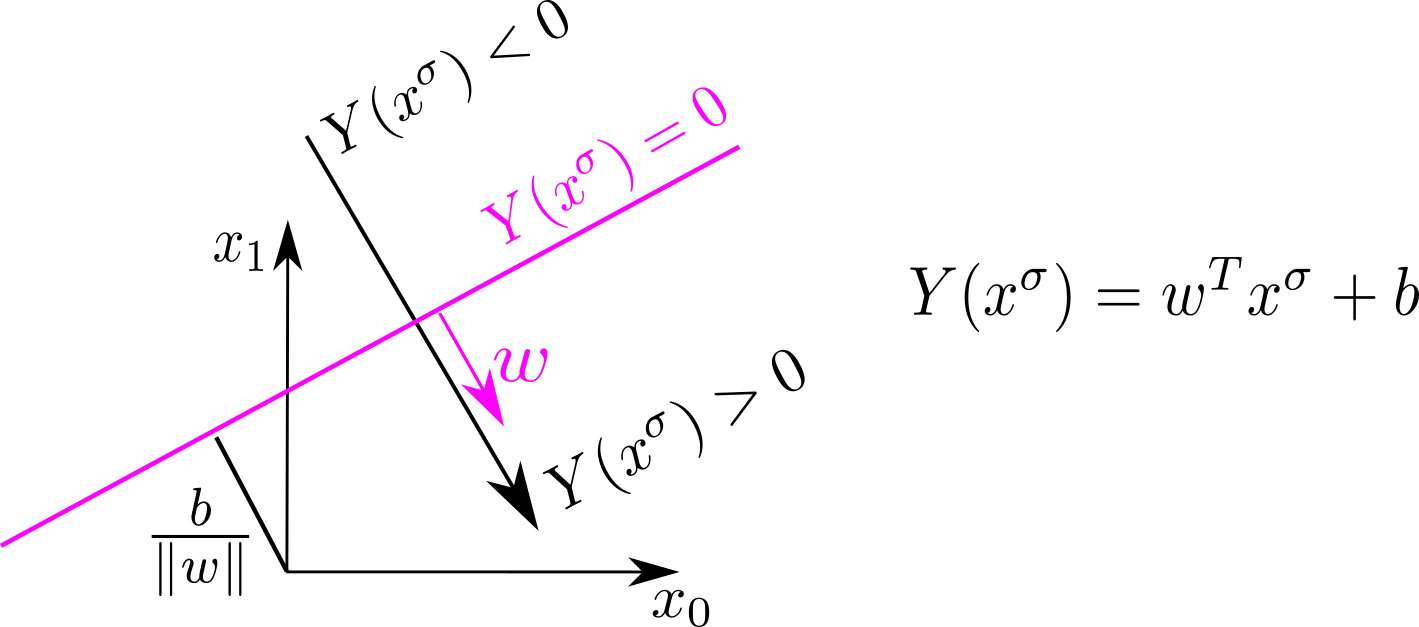
\includegraphics[width=3.5in]
{svm/svm-linear.png}
\caption{Graph of line  $Y(x^\s)=0$
splits plane
into regions with $Y<0$,
$Y=0$ and $Y>0$.} 
\label{fig-svm-linear}
\end{figure}

So far, we have 
discussed the SVM method 
for an arbitrary kernel.
This section is devoted to
the {\bf Linear (aka dot-product) Kernel}.
Said kernel is defined as

\beq
K(x^\s, x^{\s_0})=
(x^\s)^T x^{\s_0}
\;.
\eeq

For this kernel,
Eq.(\ref{eq-yy-x-sig})
specializes to


\beqa
Y(x^{\s_0})
&=&
\sum_\s \alp^\s y^\s K(x^\s, x^{\s_0}) + b
\\
&=& w^Tx^{\s_0} + b
\eeqa
where

\beq
w=\sum_\s \alp^\s y^\s x^\s
\label{eq-svm-w}
\;.
\eeq

\begin{figure}[h!]
\centering
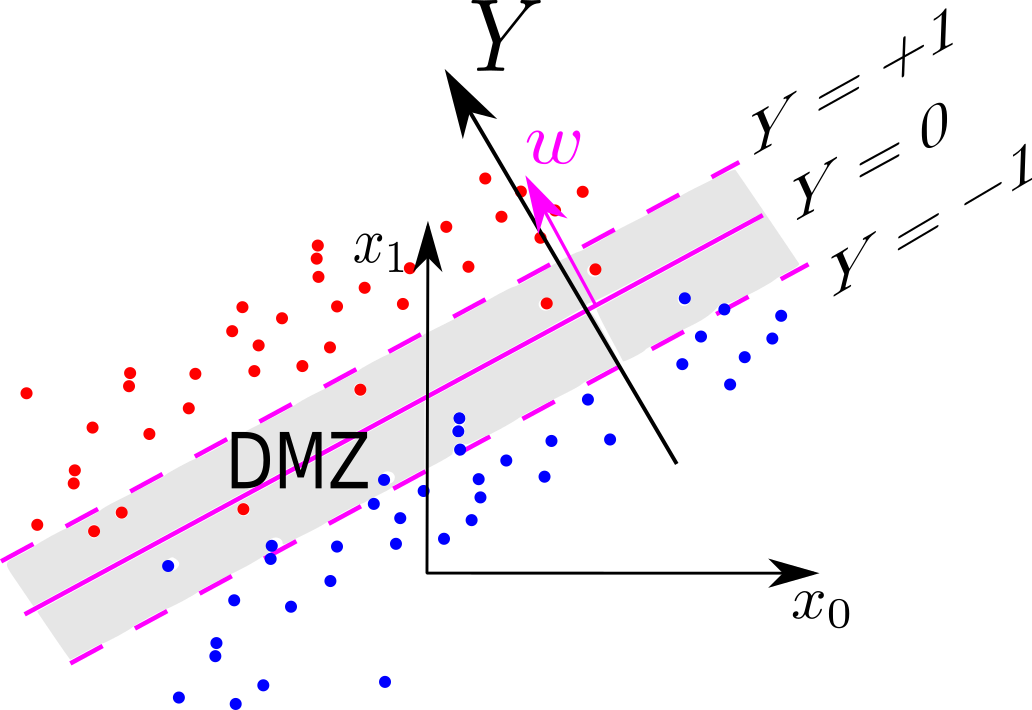
\includegraphics[width=3.5in]
{svm/svm-dmz.png}
\caption{We refer to the gray shaded region
with $-1<Y<1$, where $Y= w^T x +b$,  
as the DMZ.}
\label{fig-svm-dmz}
\end{figure}

We started this
chapter by pulling the SVM classifier
out of a hat. We did give
reasons why it works, but we did not derive
it from a more general minimization
principle. Such a derivation
is possible, at least in the 
linear kernel case, and we give it next.


Consider the following 3 straight lines:
\beqa
w^Tx^\s + b = +A
\\
w^Tx^\s + b = 0
\\
w^Tx^\s + b = -A
\eeqa
where $w, x^\s\in \RR^{nf}$, and $b,A\in \RR$.
We can re-scale the vector $w$ and 
scalar $b$ so as to get rid of the $A$.
(i.e., replace $w\rarrow wA$ and $b\rarrow bA$
and divide common factor $A$ out of equations).
This rescaling does not
affect the graphs (i.e., $x$ loci)
of these 3 lines. Now we have:


\beqa
w^Tx^\s + b = +1
\\
w^Tx^\s + b = 0
\\
w^Tx^\s + b = -1
\eeqa
If $Y$ stands for

\beq
Y=w^Tx^\s + b
\;,
\eeq
then we define
the {\bf DMZ (demilitarized zone)}
to be the region 

\beq
DMZ=\{  x^\s: |Y(x^\s)|<1\}
\;.
\eeq
The lines $Y=\pm 1$
will be called the {\bf borders (aka margins)}
of the DMZ, and 
line $Y=0$
will be called the
{\bf line of demarcation}
of the DMZ.
The DMZ is illustrated in Fig.\ref{fig-svm-dmz}.

Let $D_{DMZ}$ be
the {\bf DMZ width} (i.e., 
the distance from one border
of the DMZ to the other.)
Position vectors 
 pointing 
from the origin to either 
of the two DMZ borders are called 
{\bf support vectors}.
Suppose $X^+, X^-\in \RR^{nf}$
are two support vectors
on  opposite DMZ borders
with $|X^+-X^-|=D_{DMZ}$. Then 

\beqa
w^T X^+ + b = 1
\\
w^T X^- + b = -1
\eeqa
so

\beq
D_{DMZ}= \frac{2}{|w|}
\;.
\eeq

For any $a\in \RR$, let 
the {\bf positive $a_+$ 
and negative $a_-$
parts of $a$} be
given by

\beq
a= 
\underbrace{a_+}_
{ a\indi(a>0)} 
+ 
\underbrace{a_-}_
{ a\indi(a\leq 0)}
\;.
\eeq
\begin{figure}[h!]
\centering
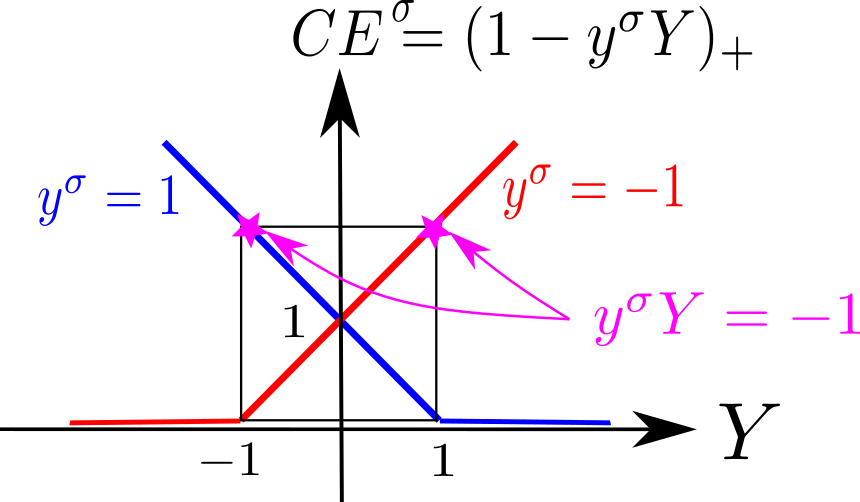
\includegraphics[width=2.5in]
{svm/svm-hinge.png}
\caption{Plot of $CE^\s$ versus $Y$.} 
\label{fig-svm-hinge}
\end{figure}

When $Y=\pm 1$,
an  error in $Y(x^\s)$  occurs iff $y^\s Y(x^\s)=-1$.
But how should we define
errors when $Y$ is a real number?
Define the {\bf Cost of erring for sample $\s$} to be

\beqa
CE^\s(x^\s, y^\s)
&=&
(1-y^\s Y(x^\s))_+
\;.
\eeqa

$CE^\s$ is shown in Fig.\ref{fig-svm-hinge}.
As you can see, 
there is a penalty for living on the
incorrect side, 
and even a penalty for living on the 
correct side but too close to the DMZ.

Note that the line of demarcation
should have the lowest $CE^\s$
for all possible $w, b$. So to find
that line,
we want to minimize  $CE^\s$
with respect to $w, b$.
But note that $CE^\s\geq 0$, 
and it can be zero for an appropriately
chosen $w$. So we need to add another 
cost in order to get a non-zero total cost.
Define the {\bf DMZ cost} as 

\beq
CZ=\frac{1}{2}|w|^2=
\frac{2}{D_{DMZ}^2}
\eeq
Note that $CZ\rarrow \infty$
as $D_{DMZ}\rarrow 0$,
so $CZ$ penalizes DMZ's that are too narrow.

Now define a Lagrangian $\call$
to be the sum 
of these 2 contributions.
\beqa
\call&=& CZ + \sum_\s CE^\s
\\
&=&
 \frac{1}{2} |w|^2 + \sum_\s (1-y^\s Y(x^\s))_+
\eeqa
This particular choice of $CZ$
is not unique, but it isn't totally arbitrary either. 
We want it to be independent of the sample $\s$,
and to depend on a geometrical aspect of the DMZ,
 like its width $D_{DMZ}=2/|w|$.
Note that $CE^\s$ behaves, when $|w|\rarrow \infty$,
 linearly in $|w|$.
We are going to differentiate $\call$ with 
respect to $|w|$
to find an optimum.
But straight lines have no optima, so we need
$CZ$ to behave, when $|w|\rarrow \infty$,
  as $|w|^p$ for some 
integer $p>1$.



Setting the variation $\delta \call$
to zero, we get

\beq
0=\delta \call
=\delta w_i
\left\{w_i -\sum_\s
\indi(y^\s Y(x^\s)<1)y^\s x^\s_i
\right\}
\eeq
so

\beq
 w =\sum_\s
\underbrace{\indi(y^\s Y(x^\s)<1)}_
{\alp^\s}
y^\s x^\s
\;.
\eeq




\section{Alternatives to Linear Kernel}
Sometimes it is convenient to replace
the dot-product kernel given above by 
a different kernel.
Other popular kernels are:

\begin{itemize}
\item 
{\bf Radial Basis Function (RBF) Kernel.}
In this case,
 $K$ is a radial function; i.e., a
function that depends only on 
the magnitude (radius, Euclidean distance,
$L^2$ norm) of a vector. An example of an RBF kernel is the
{\bf Gaussian Kernel}

\beq
K(x^\s, x^{\s_0})=
e^{ -\gamma |x^\s-x^{\s_0}|^2}
\eeq
for some free parameter $\gamma>0$.

\item
{\bf Inhomogeneous Polynomial Kernel}
\beq
K(x^\s, x^{\s_0})=
[(x^\s)^T x^{\s_0}+1]^d
\eeq
for some positive integer $d$.

\item
{\bf Homogeneous Polynomial Kernel}
\beq
K(x^\s, x^{\s_0})=
[(x^\s)^T x^{\s_0}]^d
\eeq
for some positive integer $d$.


\item
{\bf "Kernel trick" Kernel.}
Consider a map $\Phi:\RR^{nf}\rarrow \RR^N$.
Usually $N>nf$. $\Phi$ can be a
rectangular matrix 
$A\in\RR^{N\times nf}$
so that $\Phi(x^\s)=Ax^\s\in \RR^N$. Let



\beq
K(x^\s, x^{\s_0})=
[\Phi(x^\s)]^T\Phi(x^{\s_0})
\eeq
Although the constant surfaces  of 
this kernel are
hyperplanes in $\RR^N$,
its constant
surfaces in $\RR^{nf}$
can be curved and even closed 
compact surfaces (e.g. spheres).

\end{itemize}

\section{Random Forest and Kernel Method}
